% Modified based on Xiaoming Sun's template and https://www.overleaf.com/latex/templates/cs6780-assignment-template/hgjyygbykvrf

\documentclass[a4 paper,12pt]{article}
\usepackage[inner=2.0cm,outer=2.0cm,top=2.0cm,bottom=2.0cm]{geometry}
\linespread{1.1}
\usepackage{setspace}
\usepackage[rgb]{xcolor}
\usepackage{verbatim}
\usepackage{subcaption}
\usepackage{fancyhdr}
\usepackage{fullpage}
\usepackage[colorlinks=true, urlcolor=blue, linkcolor=blue, citecolor=blue]{hyperref}
\usepackage{booktabs}
\usepackage{amsmath,amsfonts,amsthm,amssymb}
\usepackage[shortlabels]{enumitem}
\usepackage{setspace}
\usepackage{extramarks}
\usepackage{soul,color}
\usepackage{graphicx,float,wrapfig}
\newenvironment{breakablealgorithm}
  {% \begin{breakablealgorithm}
   \begin{center}
     \refstepcounter{algorithm}% New algorithm
     \hrule height.8pt depth0pt \kern2pt% \@fs@pre for \@fs@ruled
     \renewcommand{\caption}[2][\relax]{% Make a new \caption
       {\raggedright\textbf{\ALG@name~\thealgorithm} ##2\par}%
       \ifx\relax##1\relax % #1 is \relax
         \addcontentsline{loa}{algorithm}{\protect\numberline{\thealgorithm}##2}%
       \else % #1 is not \relax
         \addcontentsline{loa}{algorithm}{\protect\numberline{\thealgorithm}##1}%
       \fi
       \kern2pt\hrule\kern2pt
     }
  }{% \end{breakablealgorithm}
     \kern2pt\hrule\relax%
   \end{center}
  }
\makeatother
\newtheoremstyle{definitionstyle}
  {3pt} % Space above
  {3pt} % Space below
  {\normalfont} % Body font
  {} % Indent amount
  {\bfseries} % Theorem head font
  {} % Punctuation after theorem head
  { } % Space after theorem head
  {} % Theorem head spec (can be left empty, meaning `normal`)

\theoremstyle{definitionstyle}
\newtheorem{defn}{Definition}
\newtheorem{thm}{Theorem}
\newtheorem{lem}{Lemma}
\newtheorem{statement}{Statement}
% \newtheorem{proof}{Proof}
\usepackage{framed}
\newenvironment{framedminipage}
    {\begin{framed}\begin{minipage}{0.9\textwidth}}
    {\end{minipage}\end{framed}}
\newcommand{\homework}[3]{
	\pagestyle{myheadings}
	\thispagestyle{plain}
	\newpage
	\setcounter{page}{1}
	\noindent
	\begin{center}
		\framebox{
			\vbox{\vspace{2mm}
				\hbox to 6.28in { {\bf Deep Learning \hfill} {\hfill {\rm #2} {\rm #3}} }
				\vspace{4mm}
				\hbox to 6.28in { {\Large \hfill #1  \hfill} }
				\vspace{3mm}}
		}
	\end{center}
	\vspace*{4mm}
}
\newcommand\numberthis{\addtocounter{equation}{1}\tag{\theequation}}

\begin{document}
\homework{HW2}{2024011303}{Liu Hanzuo}
\section*{True or False}
\paragraph{P1} False; Whether $q_\theta$ collapse to all multimodal depends on whether the KL divergence is inclusive or exclusive.
\paragraph{P2} True; Randomness of sampling has been moved to the randomness of $\epsilon$ in the equation of 
\[
    z=\mu+\sigma\cdot\epsilon, \epsilon\sim\mathcal{N}(0,1)
\]
\paragraph{P3} False; we need a nueral network $q_\phi(z)$ to approximate the posterior distribution $p(z|x)$.
\paragraph{P4} False; a larger $\beta$ indicated the variables to be more independent.
\section*{QA}
\paragraph{P5} We begin by show a equation
\begin{framedminipage}
\begin{lem}
\[
  KL(q(z)||p(z|x))=\log p(x)-\sum_z q(z)\log\frac{p(z,x)}{q(z)}
\]
\end{lem}
\end{framedminipage}
\begin{proof}
\[
  KL(q(z)||p(z|x))=\sum_z q(z)\log\frac{q(z)}{p(z|x)}=\sum_z q(z)\log\frac{q(z)p(x)}{p(z,x)}
\]
\[
  =\sum_z q(z)\log p(x)-\sum_z q(z)\log\frac{p(z,x)}{q(z)}=\log p(x)-\sum_z q(z)\log\frac{p(z,x)}{q(z)}
\]
\end{proof}
Thus, we have
\[
  F(\theta,q)=\sum_z q(z)\log p_\theta(x,z)-\sum_z q(z)\log q(z)
\]
\[
  =\sum_z q(z)\log\frac{p(z,x)}{q(z)}=\log p(x)-KL(q(z)||p(z|x))
\]
To maximize $q$, it's equivalent to minimize $KL(q(z)||p(z|x))$, thus $q(z)\leftarrow p(z|x)$ is equivalent to the E-step.\\
For the M-step
\[
  \arg\max_\theta F(\theta,q^t)=\mathbb{E}_{z\sim p^t_\theta(z|x)}\left[\log p_\theta(x,z)\right]+H(p^t_\theta(x|z))=\arg\max_\theta Q(\theta|\theta^t)+H(p^t_\theta(x|z))
\]
Since when maximizing $\theta$ part, $H(p^t_\theta(x|z))$ is a constant, thus 
\[
  \arg\max_\theta F(\theta,q^t)=\arg\max_\theta Q(\theta|\theta^t)
\]
Thus we prove the equivalent of two updating policy.
\paragraph{P6} 
\textbf{1.}
\begin{proof}
\[
  KL(N_0||N_1)=\mathbb{E}_{N_0}\left[\log\frac{N_0(x)}{N_1(x)}\right]
\]
Now we write down two PDFs:
\[
  N_0(x)=\frac{1}{(2\pi)^{\frac{d}{2}}|\Sigma_0|^{\frac{1}{2}}}\exp\left(-\frac{1}{2}(x-\mu_0)^T\Sigma_0^{-1}(x-\mu_0)\right)
\]
\[
  N_1(x)=\frac{1}{(2\pi)^{\frac{d}{2}}|\Sigma_1|^{\frac{1}{2}}}\exp\left(-\frac{1}{2}(x-\mu_1)^T\Sigma_1^{-1}(x-\mu_1)\right)
\]
The log ratio could be written as:
\[
  \log\frac{N_0(x)}{N_1(x)}=\log\frac{|\Sigma_1|^{\frac{1}{2}}}{|\Sigma_0|^{\frac{1}{2}}}-\frac{1}{2}(x-\mu_0)^T\Sigma_0^{-1}(x-\mu_0)+\frac{1}{2}(x-\mu_1)^T\Sigma_1^{-1}(x-\mu_1)
\]
\[
  KL(N_0||N_1)=\mathbb{E}_{N_0}\left[\log\frac{N_0(x)}{N_1(x)}\right]
\]
\[
  =\log\frac{|\Sigma_1|^{\frac{1}{2}}}{|\Sigma_0|^{\frac{1}{2}}}-\frac{1}{2}\mathbb{E}_{N_0}\left[(x-\mu_0)^T\Sigma_0^{-1}(x-\mu_0)\right]+\frac{1}{2}\mathbb{E}_{N_0}\left[(x-\mu_1)^T\Sigma_1^{-1}(x-\mu_1)\right] \numberthis
\]
For calculation, we note that:
\[
  \mathbb{E}_{N_0}\left[(x-\mu_0)^T\Sigma_0^{-1}(x-\mu_0)\right]=tr(\Sigma_0^{-1}\Sigma_0)=d \numberthis
\]
let $\delta=\mu_0-\mu_1$
\[
  (x-\mu_1)^T\Sigma_1^{-1}(x-\mu_1)=(x-\mu_0+\mu_0-\mu_1)^T\Sigma_1^{-1}(x-\mu_0+\mu_0-\mu_1)
\]
\[
  =\mathbb{E}_{N_0}\left[(x-\mu_0)^T\Sigma_1^{-1}(x-\mu_0)\right]+\delta^T\Sigma_1^{-1}\delta=tr(\Sigma_1^{-1}\Sigma_0)+\delta^T\Sigma_1^{-1}\delta \numberthis
\]
Bring these euqations ((2),(3)) back to the KL divergence ((1)), we have:
\[
  KL(N_0||N_1)=\frac{1}{2}\left[\log\frac{|\Sigma_1|}{|\Sigma_0|}-d+tr(\Sigma_1^{-1}\Sigma_0)+(\mu_1-\mu_0)^T\Sigma_1^{-1}(\mu_1-\mu_0)\right] 
\]
\end{proof}
\textbf{2.} 
\begin{proof}
We only need to show that $\forall p_1,p_2,q_1,q_2$, we have:
\[
  \left(\lambda p_1+(1-\lambda)p_2\right)\log\frac{\left(\lambda p_1+(1-\lambda)p_2\right)}{\lambda q_1+(1-\lambda)q_2}\le\lambda p_1\log\frac{p_1}{q_1}+(1-\lambda)p_2\log\frac{p_2}{q_2}
\]
Then taking the interval over all $x$, we could get the initial inequality proved.\\
\[
  F(p_1,p_2,q_1,q_2):=\lambda p_1\log\frac{p_1}{q_1}+(1-\lambda)p_2\log\frac{p_2}{q_2}-\left(\lambda p_1+(1-\lambda)p_2\right)\log\frac{\left(\lambda p_1+(1-\lambda)p_2\right)}{\lambda q_1+(1-\lambda)q_2}
\]
Note that 
\[
  \frac{\partial}{\partial q_1}F(p_1,p_2,q_1,q_2)=-\lambda p_1\frac{1}{q_1}+\left(\lambda p_1+(1-\lambda)p_2\right)\frac{1}{\lambda q_1+(1-\lambda)q_2}
\]
From Lagrange multiplier, we have:
\[
  \frac{p_1}{q_1}=\frac{p_2}{q_2}:=k
\]
(Notation: this equation could also obtained from considering the minimum point for a singular variable $q_1$)\\
At this assumption, we have that:
\[
  LHS=\left(\lambda p_1+(1-\lambda)p_2\right)\log k=RHS
\]
Thus we have proved the inequality.
\end{proof}
\textbf{3.} Here we show the exclusive and inclusive KL divergence example.\\
\begin{figure}[H]
  \centering
  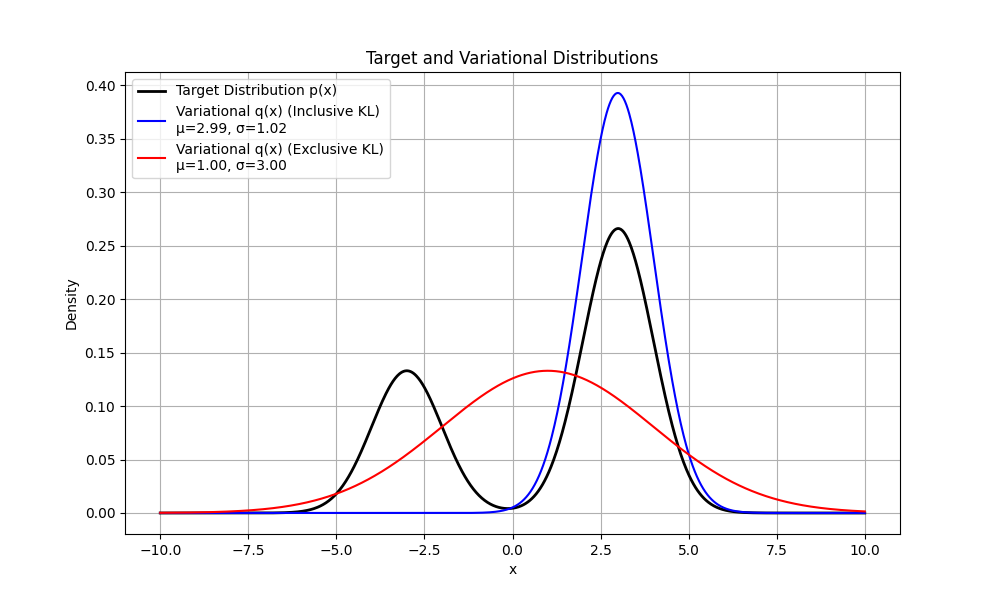
\includegraphics[width=\textwidth]{6-3.png}
  \caption{Figure 6-3: Exclusive and Inclusive KL divergence}
  \label{fig:6-3}
\end{figure}
\textbf{4.} The objective is:
\[
  \mathbb{E}_{z\sim p(z|x)}[\log\frac{p(z|x)}{q_\phi(z|x)}]
\]
Note that though the optimal $q_\phi(z|x)$ is $p(z|x)$, there is pros and cons to take the inclusive KL divergence.\\
\textbf{Pros:}
\begin{enumerate}
  \item $q_\phi(z|x)$ will tend to cover all possible areas that $p(z|x)>0$, having a relative large penalty if $p(z|x)>0$ but $q_\phi(z|x)=0$. (Which indicate that $q_\phi(z|x)$ need to cover all modules and possible areas that $p(z|x)>0$)
  \item $q_\phi(z|x)$ will have a diverge result, cover larger areas
\end{enumerate}
\textbf{Cons:}
\begin{enumerate}
  \item $q_\phi(z|x)$ have a non-accurate probability distribution due to a diverge result, lower confidence over the high probability $p(z|x)$ result.
  \item Hard to sample from the posterior distribution $z\sim p(z|x)$, larger variance for gradients.
  \item Waste probability in low probability areas.
\end{enumerate}
Theoretically, we could also gain the similar expression:
\[
  KL(p(z|x)||q_\phi(z))=\sum_z p(z|x)\log\frac{p(z|x)}{q_\phi(z)}=\sum_z p(z|x)\log\frac{p(z,x)}{q_\phi(z)p(x)}
\]
\[
  =-\sum_z p(z|x)\log\frac{q_\phi(z)}{p(z,x)}-\log p(x)=-\frac{1}{p(x)}\sum_z p(z,x)\log\frac{q_\phi(z)}{p(z,x)}-\log p(x)
\]
Thus we have:
\[
  -\log p(x)=KL(p(z|x)||q_\phi(z))+\frac{1}{p(x)} ELBO  
\]
While, does not have the beautiful formula that the exclusive KL divergence has.
\paragraph{P7}
\textbf{1.}
\[
  \log p_{\mu,\sigma,\theta}(x)\ge\mathbb{E}_{w,z\sim q_{\psi,\phi}(w,z|x)}\left[\log \frac{p(w,z,x)}{q_{\psi,\phi}(w,z|x)}\right]=ELBO
\]
Thus we have:
\[
  ELBO=\sum q_\psi(w|x)q_\phi(z|w,x)\log\frac{p(w,z,x)}{q_\psi(w|x)q_\phi(z|w,x)}
\]
\[
  =\mathbb{E}_{q(w,z|x)}\left[\log p_\theta(x|w)\right] 
  + \mathbb{E}_{q(w,z|x)}\left[\log p_{\mu,\sigma}(w|z)\right] 
  + \mathbb{E}_{q(w,z|x)}\left[\log p(z)\right] 
\]
\[
  - \mathbb{E}_{q(w,z|x)}\left[\log q_\psi(w|x)\right] 
  - \mathbb{E}_{q(w,z|x)}\left[\log q_\phi(z|w,x)\right]
\]
\[
  =\mathbb{E}_{w\sim q_\psi(w|x)}\left[\log p_\theta(x|w)\right] 
  - \mathbb{E}_{w\sim q_\psi(w|x)}\left[KL(q_\phi(z|w,x) \| p(z))\right] 
  - KL(q_\psi(w|x) \| \mathbb{E}_{z \sim p(z)}[p_{\mu,\sigma}(w|z)]) 
\]
\textbf{2.}
\begin{enumerate}
\item Here we calculate the result of different term in the loss function.
\[
  \mathbb{E}_{q(w,z|x)}\left[\log p_\theta(x|w)\right]=\mathbb{E}_{q(w,z|x)}\left[-\log\det\sigma_\theta(w)+\frac{(x- \mu_\theta(w))^T*\sigma_\theta(w)^{-2}(x- \mu_\theta(w))}{2}\right]+Const
\]
\item If we have the closed form easy-calculating $q(w,z|x)$ (such as Gaussian), we could use the reparameterization trick to calculate the expectation and expectation.
\[
  \mathbb{E}_{w\sim q_\psi(w|x)}\left[KL(q_\phi(z|w,x) \| p(z))\right]= \mathbb{E}_{w\sim q_\psi(w|x)}\sum_{k=1}^K q_\phi(k|w,x)\log\frac{q_\phi(k|w,x)}{\pi_k}
\]
Could use reparameterization trick: 
\[
  x = \mu_\theta(w) + \sigma_\theta(w) \cdot \epsilon, \epsilon \sim \mathcal{N}(0, I)
\]
\[
  w = \mu_z + \sigma_z \cdot \epsilon, \epsilon \sim \mathcal{N}(0, I)
\]
to back propogate the gradients.
\item the third term could be written as:
\[
  KL(q_\psi(w|x) \| \mathbb{E}_{z \sim p(z)}[p_{\mu,\sigma}(w|z)]) = 
\mathbb{E}_{w \sim q_\psi(w|x)} \left[ \log q_\psi(w|x) - \log \mathbb{E}_{z \sim p(z)}[p_{\mu,\sigma}(w|z)] \right]
\]
\[
  =\mathbb{E}_{w \sim q_\psi(w|x)}\left[ \log q_\psi(w|x) - \log\sum_{k=1}^K \pi_k \frac{1}{\sqrt{2\pi}\sigma_k}e^{-\frac{(x-\mu_k)^2}{2\sigma_k^2}}\right]
\]
Could also be back-propogated by reparameterization trick!
\end{enumerate}
To summarize, we show that all the terms in the loss function could be back-propogated by reparameterization trick.
For the training procedure, we divide it into two parts:
\begin{itemize}
  \item back-propogate the gradients of $\log p_{\mu,\sigma,\theta}(x|w)$ to $\mu,\sigma,\theta$
  \item back-propogate the gradients of $\log p_{\mu,\sigma,\theta}(x|w)$ to $\psi,\phi$ by setting $q(w,x|x)=q_\psi(w|x)\cdot q_\phi(z|w,x)\leftarrow p(w,z|x)$ use the loss of ELBO and back-propogate the gradients using reparameterization trick.
\end{itemize}
\end{document}
